\section{Testscenario} \label{k51}

Her følger en beskrivelse av webapplikasjonen migrasjon med DBUpgradinator blir testet på. Nettbutikken ''WebShop'' benytter nøkkelverdi\-lageret Project Voldemort for å lagre et register over sine kunder. De fleste kundene av nettbutikken bor enten i Storbritannia eller i Australia. Aggregatene som lagres av Voldemort er flate, og består av strengnøkler og strengverdier.

\begin{figure}[hbtp]
    \centering
    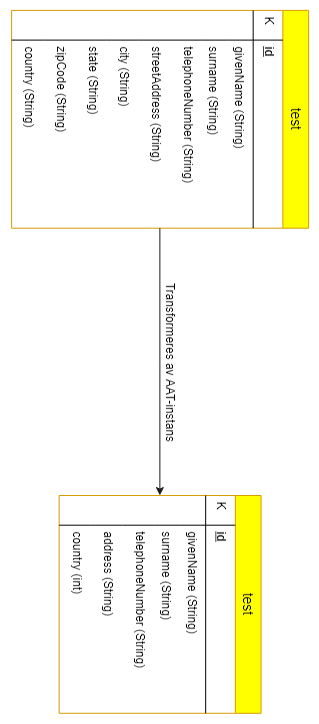
\includegraphics[scale=0.9]{fig/WSS-AggregatModell.png}
    \caption{Datamodeller for aggregatene til skjemaversjon ''x'' og dets etterfølger, ''y''.}
    \label{fig11}
\end{figure}

I skjemaversion ''x'', vist i venstre modell i figur \ref{fig11}, har aggregatene til WebShop følgende attributter: \texttt{givenName} (fornavn), \texttt{surName} (etternavn), \texttt{telephoneNumber} (telefonnummer), \texttt{streetAddress} (gateadresse), \texttt{city} (poststed), \texttt{state} (delstat - for australske og eventuelt amerikanske kunder), \texttt{zipCode} (postkode, hvis system varierer fra land til land), og \texttt{country} (landet til adressen).

Samtlige attributter er strenger, og deres verdier er også strenger. Dette er det enkleste alternativet for å representere tekst som inneholder mellomrom, bindestrek og parantes, hvilket er tilfelle for telefonnummeret og postkoden.

For amerikanske og australske kunder av WebShop er skjema ''x'' en optimal aggregatstruktur, fordi alle har en leveringsadresse bestående av både en gateadresse, poststed, delstat, postkode og land. For kunder i Storbritannia eller Irland vil delstats-feltet måtte stå tomt.

Derfor blir følgende endring gjort: Adressekomponentene \texttt{streetAddress}, \texttt{city}, \texttt{state}, \texttt{zipCode} og \texttt{country} slås sammen til ett, helhetlig adressefelt, slik at hver enkelt kunde selv kan skrive inn sin korrekte, internasjonale postadresse i en tekstboks, der hver adressekomponent står på sin egen linje. Alle de nevnte individuelle attributtene, bortsett fra én, slettes fra aggregatstrukturen.

Feltet \texttt{country} endres i stedet for å slettes. I stedet for å lagre en streng som identifiserer et land på en forkortelse, brukes i stedet en landskode, et heltall\footnote{For enkelte selvstendige stater går det ikke an å representere deres landskode med bare et heltall, da deres kode inneholder ''-''. Eksmpler på slike stater inkluderer Jamaica (1-876), Trinidad og Tobago (1-868) og Bahamas (1-242).} man må ta i bruk hvis man skal ringe en person hvis telefoniabonnement er registrert i utlandet. Først skrives et plusstegn (''+''), etterfulgt av landskoden og deretter personens telefonnummer. Skjemaendringen blir gjort fordi de færreste brukere skriver inn landskoden sammen med telefonnummeret sitt i et tekstfelt når de registrert. Den typiske netthandel utleder istedet brukerens landskode utifra deres oppgitte land.

Denne skjemaoppgraderingen består av to endringer som gjør at det nye skjemaet, ''y'', ikke er bakoverkompatibelt med skjema ''x''. For det første endres typen til ett attributt fra streng til heltall. Denne endringen er inkompatibel skjemaene imellom, fordi mengden gyldige strenger er uendelig større enn mengden gyldige heltall.

Den andre kompabilitetsbrytende endringen er at ett eller flere attributter slettes. Se kodeoppføring \ref{uat} for kildekode som oppretter et nytt aggregat basert på aggregatet \texttt{val}, som tilhører det gamle skjemaet. Her brukes en tredjeparts modul til å forme JSON-strenger uten at metoden har noe direkte informasjon om parameteret \texttt{val}, som er en streng.

\newpage
\begin{lstlisting}[language=Java, label=uat, caption={Transformasjonsklasse for aggregat som holdeer data om registrerte brukere i WebShop.}]
package app;

import org.json.JSONObject;
import vbb.dbupgradinator.AbstractAggregateTransformer;

public class UserAggregateTransformer extends AbstractAggregateTransformer {

    public UserAggregateTransformer(String current, String next) {
        super(current, next);
    }

    private static String checkEmptyness(String d) {
        if (d.isEmpty()) { return ""; }
        return d + "\n";
    }

    private static int getCountryCode(String country) {
        int phone = -1;
        String checker = country.toUpperCase();
        if (checker == "UK") { phone = 44; }
        else if (checker == "AUS") { phone = 61; }
        return phone;
    }

    public String transformAggregate(String val) {
      JSONObject jo = new JSONObject(val);
      String countryAbb = jo.getString("country");
      String fullAddress = checkEmptyness(jo.getString("streetAddress")) + checkEmptyness(jo.getString("city")) + checkEmptyness(jo.getString("state")) + checkEmptyness(jo.getString("zipCode")) + checkEmptyness(countryAbb);
      jo.put("address", fullAddress);
      jo.remove("streetAddress");
      jo.remove("city");
      jo.remove("state");
      jo.remove("zipCode");
      jo.put("country", getCountryCode(countryAbb));
      return jo.toString();
    }
}
\end{lstlisting}


